\subsection{First Experience}

\subsubsection{URL to IP address using DNS}
After pinging www.icann.net on both NixOS and Windows 11, respectively, we
obtained two different IP addresses, one IPv4 and one IPv6.

\begin{figure}[htbp]
    \centering
    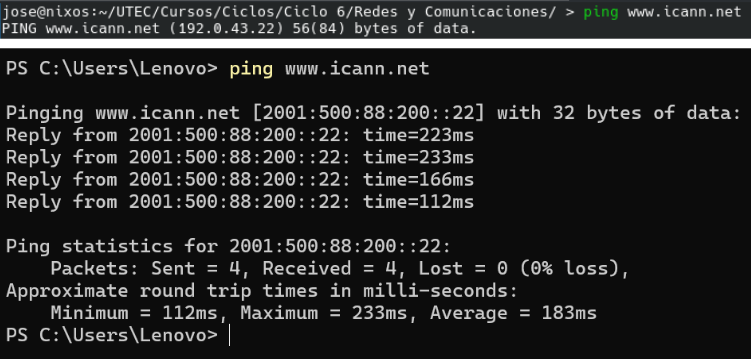
\includegraphics[width=1\linewidth]{img/1.png}
    \caption{www.icann.net addresses}\label{fig:1}
\end{figure}

We then proceeded to ping www.unsplash.com, to see if we would get different IP
addresses, which we did, as we pinged a different server. Not necessarily
because of different hostnames, as multiple hostnames could point to the same
IP address.

\begin{figure}[htbp]
    \centering
    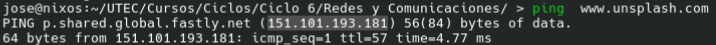
\includegraphics[width=1\linewidth]{img/2.png}
    \caption{www.unsplash.com IP address}\label{fig:2}
\end{figure}

We then tried plugging in the obtained IP address into our browsers, to see if
we could access the Unsplash webpage directly. However, the website did not
show up. After some quick research, we found out that Unsplash uses Fastly,
which works as a CDN (Content Delivery Network). This means that the address we
tried to use is not the actual address of the Unsplash website, but rather the
IP address of a Fastly server that redirects users to the actual website using
\textbf{the hostname header}.

Since we did a raw request and didn't provide the specified hostname, the
server did not know where to redirect us, and thus displayed an error.

\begin{figure}[htbp]
    \centering
    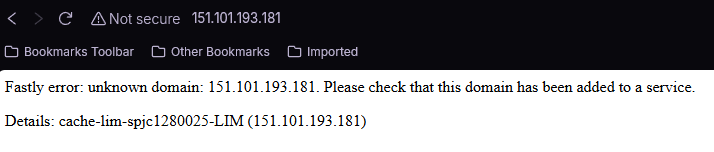
\includegraphics[width=1\linewidth]{img/3.png}
    \caption{Fastly error}\label{fig:3}
\end{figure}

\subsubsection{DNS lookup with nslookup}

After using the nslookup command with the Unsplash hostname, we got the
following output:

\begin{figure}[htbp]
    \centering
    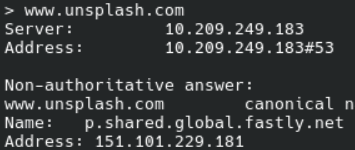
\includegraphics[width=1\linewidth]{img/4.5.png}
    \caption{nslookup output}\label{fig:4}
\end{figure}

The DNS server's IP is 10.209.249.183, and we figured must be a local DNS
server, as it belongs in the private IP range 10.x.x.x. The translated IP
address appears just below the DNS server's IP.\@ This time, it's different
from the one we got when using the ping command.

We then typed the IP address we got into another nslookup prompt, and we got
the following error:

\begin{figure}[htbp]
    \centering
    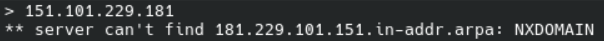
\includegraphics[width=1\linewidth]{img/5.png}
    \caption{nslookup output 2}\label{fig:5}
\end{figure}

The nslookup command expects a hostname to resolve to an IP address, and
because we gave it an IP address, it could not find the corresponding domain.

With the goal of experimenting a bit more, we repeated the experience with a
different hostname, using \textit{cisco.com}.

\begin{figure}[htbp]
    \centering
    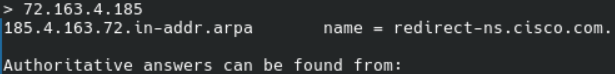
\includegraphics[width=1\linewidth]{img/6.png}
    \caption{cisco.com nslookup output}\label{fig:6}
\end{figure}

The request used the same local DNS server as before, and the resolved IP is
different from Unsplash's. We then tried using \textit{www.cisco.com} instead.

\begin{figure}[htbp]
    \centering
    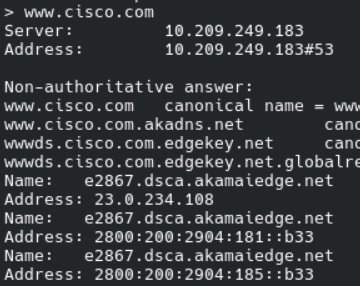
\includegraphics[width=1\linewidth]{img/7.png}
    \caption{www.cisco.com nslookup output}\label{fig:7}
\end{figure}

The output is different, as the first request used a top-level domain (TLD),
while the second one used a subdomain. Furthermore, Cisco uses CDNs, like
Unsplash, to serve their content quickly in different locations.

Finally, we tried using \textit{www.google.com}. The results are displayed
below:

\begin{figure}[htbp]
    \centering
    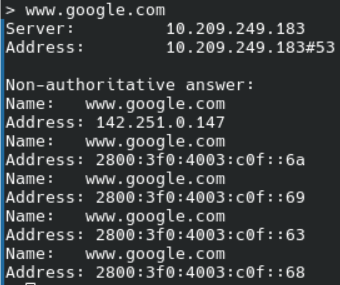
\includegraphics[width=1\linewidth]{img/8.png}
    \caption{www.google.com nslookup output}\label{fig:8}
\end{figure}

We noticed there were IP addresses that looked different and used colons
instead of dots to separate each number. These are IPv6 addresses, a newer
standard which was developed to replace IPv4. They're both used nowadays, but
IPv4 is still more common.
